%
%   Copyright 2013 Katarzyna Szawan <kat.szwn@gmail.com>
%       and Michał Rus <m@michalrus.com>
%
%   Licensed under the Apache License, Version 2.0 (the "License");
%   you may not use this file except in compliance with the License.
%   You may obtain a copy of the License at
%
%       http://www.apache.org/licenses/LICENSE-2.0
%
%   Unless required by applicable law or agreed to in writing, software
%   distributed under the License is distributed on an "AS IS" BASIS,
%   WITHOUT WARRANTIES OR CONDITIONS OF ANY KIND, either express or implied.
%   See the License for the specific language governing permissions and
%   limitations under the License.
%

\subsection{Android component}
\label{subsec:component-android}

% -------------------------------- Android

Our application consists of the following main components:

\begin{itemize}
	\item an action bar at the top of user's display; on the left side of it, there should be our application's name displayed; on the right side: action items that enable the user to create/import/close a mind map,
	\item a view with tabs, that lets the user switch between currently opened maps and a list of all maps available,
	\item a view with a list of maps available to the user consisting of vertically positioned clickable areas with map title and date of its last modification; a click/tap on such an area (re)opens a tab with proper mind map,
	\item a custom view for displaying a mind map in its tab; this contains many:\begin{itemize}
		\item mind node views consisting of a text field with node's content and a button to add children to the node,
		\item views of arrows that connect children to their parents.
	\end{itemize}
\end{itemize}

\Cref{fig:mockup-maplist} below shows a \emph{mock-up} (a sketch/plan) of the main, initial screen of the Android application. As planned, the user can:

\begin{itemize}
	\item choose an existing map to edit,
	\item select and delete a map by long-pressing it,
	\item add a new map,
	\item import an existing XMind map,
	\item switch to any other opened map using the tabs at the top.
\end{itemize}

\begin{figure}[h]
	\centering
	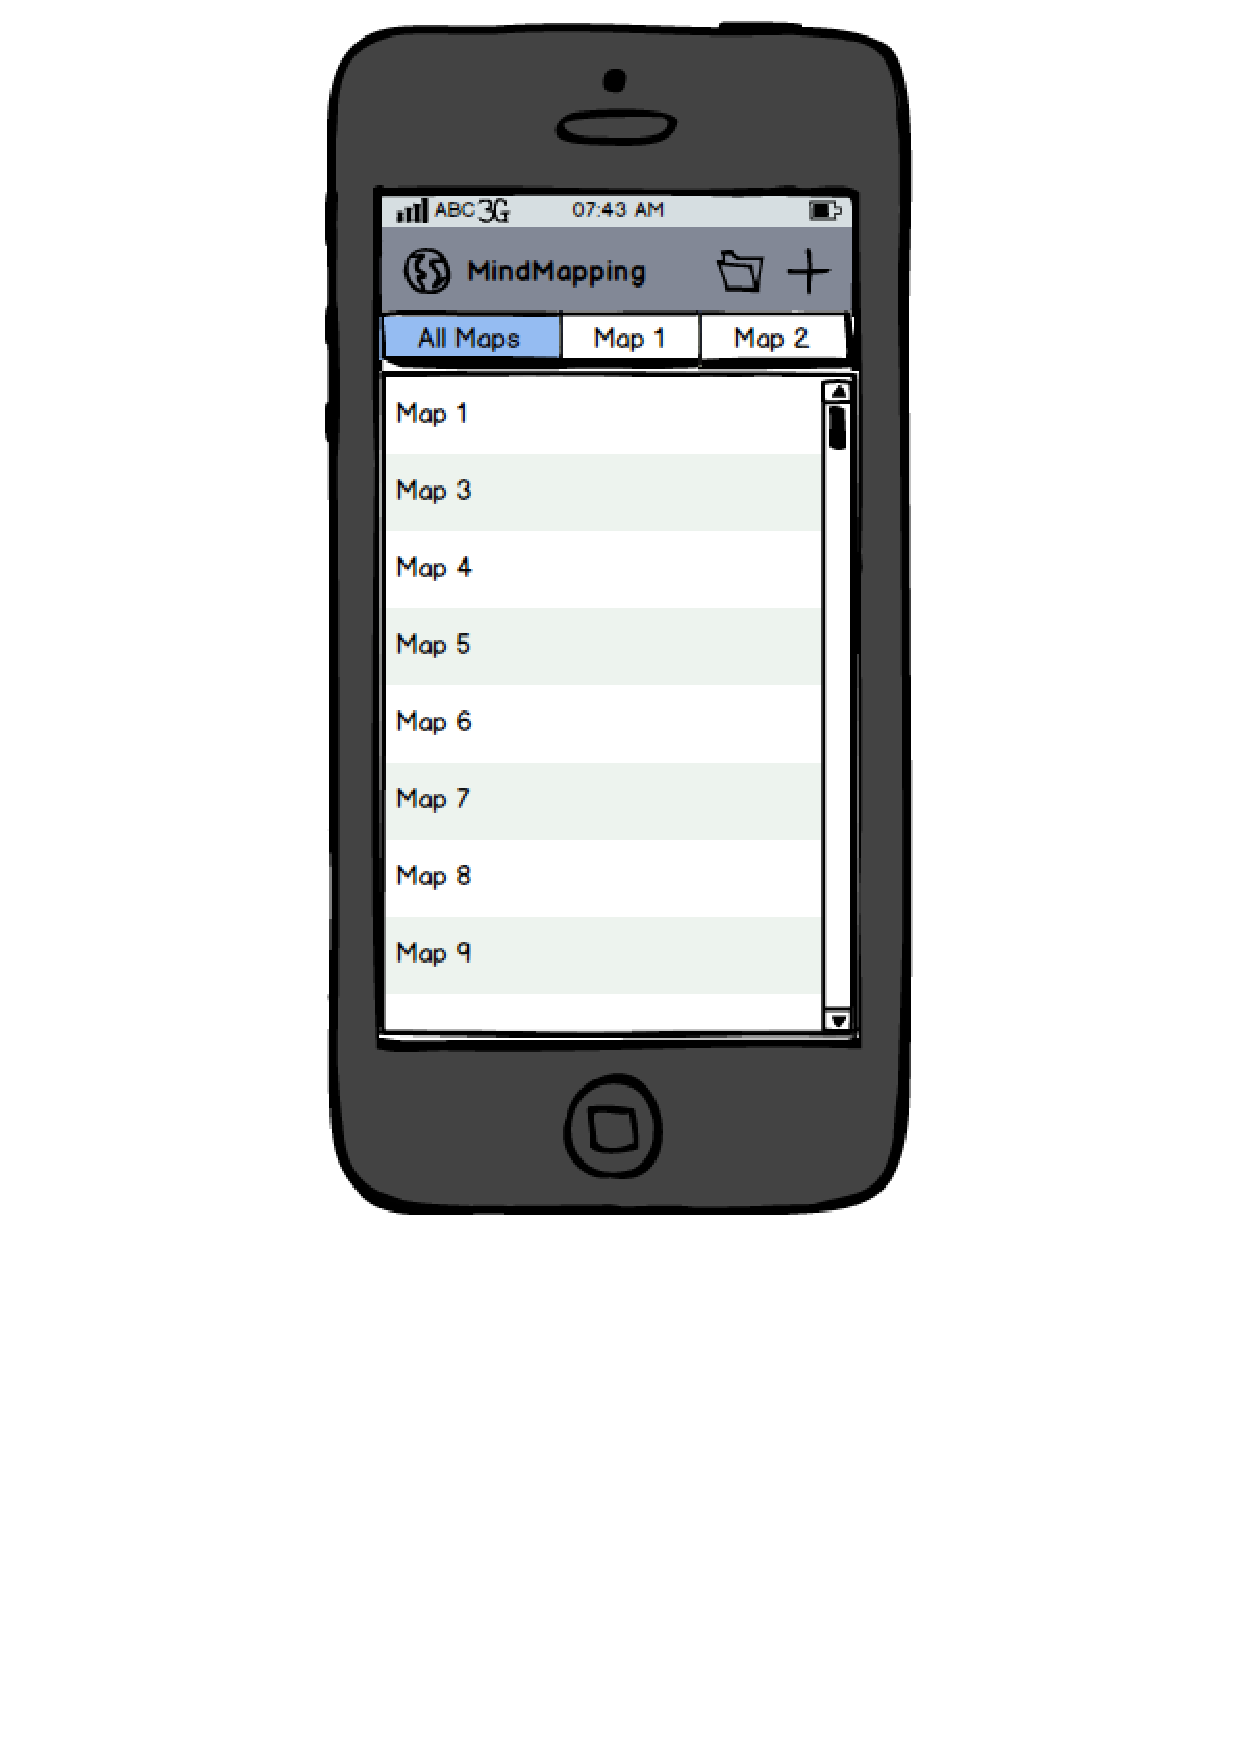
\includegraphics[width=0.5\textwidth]{graphics-mockup-list}
	\caption{Mock-up of mind map list, initial screen.}
	\label{fig:mockup-maplist}
\end{figure}

\Cref{fig:mockup-mindmap} shows a similar preview of a map view: a screen that is shown to the user when they choose/add/import a map in \cref{fig:mockup-maplist}. Here, the user can:

\begin{itemize}
	\item edit content of any `mind node' by tapping on it,
	\item remove any node (and its subtree) by long-pressing it and selecting `remove',
	\item move any node (reassign its parent node) by long-pressing it and selecting `change parent', and then tapping on the new parent,
	\item add a child node to any node by tapping on `+' button next to the parent node,
	\item see (in real-time) changes introduced by other editors currently editing this map.
\end{itemize}

\begin{figure}[h]
	\centering
	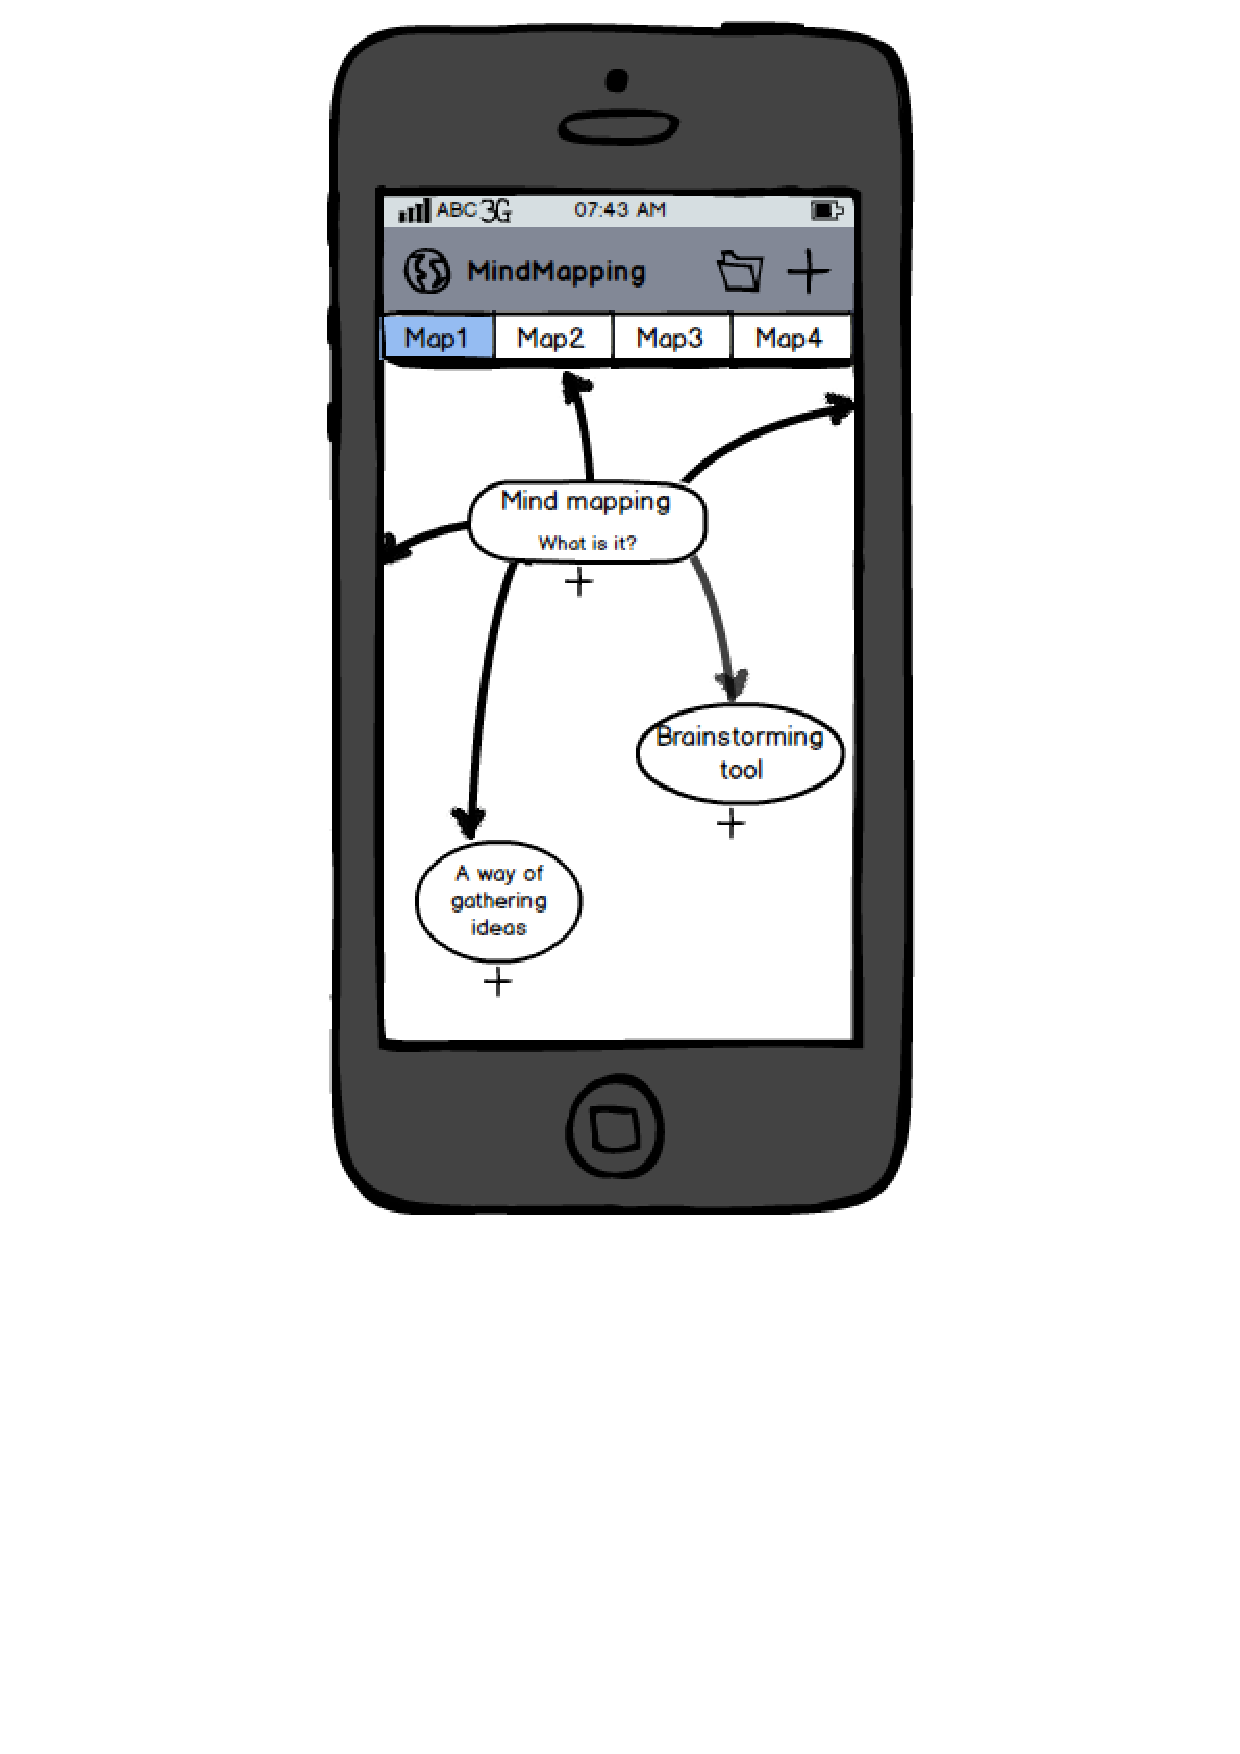
\includegraphics[width=0.5\textwidth]{graphics-mockup-map}
	\caption{Mock-up of mind map view.}
	\label{fig:mockup-mindmap}
\end{figure}


\subsection{Akka applications}
\label{subsec:proj-component-akka}
% -------------------------------- Akka

Akka, on the other hand, is used as a backend for the mobile application (and---possibly---for \emph{any other} client app yet-to-come into existence). It enables all mobile devices with the application installed to share maps and collaborate on them in real-time. Several REST web services are implemented using Spray.io (a REST interface to Akka) for communication between Android devices and actor system on the server-side.

Each REST-connected mobile device gets its own actor. Instant bidirectional communication between devices is achieved by means of `long-polling': mobile app initiates a connection with a REST service which does not respond until its actor receives a message from another actor. See \cref{subsec:android-akka-comm} for details about Android--Akka communication protocol.

Our Akka application consists of components described below.

\begin{description}
	\item[Actor system]{provided by Akka framework; an environment in which all actors (of custom and system origin) live.}
	\item[Main supervisor actor]{provided by Akka; tightly integrated with the actor system. There is always one such actor for each system.}
	\item[Squeryl]{being an object-relational mapper and domain specific language for Scala and SQL databases (including PostgreSQL). Squeryl puts great emphasis on minimum verbosity and maximum type safety, as well as Don't-Repeat-Yourself principle. Created statements are validated by Scala compiler (this includes types of field). Statements that pass compilation won't fail at runtime~\cite{Squeryl:Intro}.}
	\item[Database interfacing actor(s)]{that provide a persistence interface for per-user actors. Currently implemented using Squeryl.}
	\item[Spray.io based REST actors]{that manage connection between Android applications and per-user actors. These actors must encapsulate bidirectional message passing on a request-response style HTTP protocol. This is somewhat of a challenge, as described in \cref{subsec:problem-longpolling}.}
	\item[Per-user actors]{that represent a particular user/connection/device to the rest of the actor system each. By separation of these and REST actors, its is possible to easily add some other front-ends to the system. Now, the only front-end is the Android application.}
	\item[Managing actor for per-user actors]{which keeps track of all per-user actors and routes messages between them. If adding user privileges were planned, there would be no such actor (as it would be highly inefficient to check all the time which user should get which event). Instead, we would use so called `data streams' that particular per-user actors would subscribe to. Any message sent to the stream would then get automatically transmitted to all subscribed actors. Therefore a stream would represent a single mind map.}
\end{description}

The main means of communication is a `message'. This is the highest form of object-oriented model. No actor methods are called directly; instead, actors send and receive messages (similarily to Erlang's lightweight processes). Messages exchanged between different server-side actors in our system are listed below.

\begin{itemize}
	\item Messages from \emph{REST actors} to \emph{per-user actors}.
	\begin{description}
		\item[CreateMindMap]{when user creates/imports a new mind map on their device.}
		\item[UpdateNode]{when user updates a particular node on their device. This update might be a content update, parent change, deletion.}
	\end{description}

	\item Messages from \emph{per-user actors} to \emph{DB actors}.
	\begin{description}
		\item[CreateMindMap]{}
		\item[UpdateContent]{}
		\item[UpdateParent]{}
	\end{description}

	\item Messages exchanged between \emph{managing actor} and \emph{per-user actors}, and also forwarded from \emph{per-user actors} to \emph{REST actors}.
	\begin{description}
		\item[UpdatedNode]{used to notify managing actor and other per-user actors about a particular changed node.}
	\end{description}
\end{itemize}

Again, see \cref{subsec:android-akka-comm} for details about Android--Akka communication protocol.
